\pergunta{3. Suponha um sistema computacional com 64KB de memória principal e que utilize um
sistema operacional de 14KB que implemente alocação contígua de memória. Considere também
um programa de 80KB, formado por um módulo principal de 20KB e três módulos
independentes, cada um com 10KB,20KB e 30KB. Como o programa poderia ser executado
utilizando-se apenas a técnica de overlay?}
\\
O sistema operacional será alocado no início da memória principal, deixando
50 KB para programas em \textsl{userspace} utilizarem.  Overlay é o processo
de transferir um bloco de código de programa ou dados para a memória interna,
substituindo pelo bloco atual \cite{OxfordDictionary}.  Os blocos independentes
serão colocados na memória, um por vez para serem utilizados.  A memória
ficará organizada de acordo com a Figura \ref{OverlayPDF}.  O módulo principal
é encarregado de executar os \textsl{overlays}.

\begin{figure}[!ht]
  \centering
	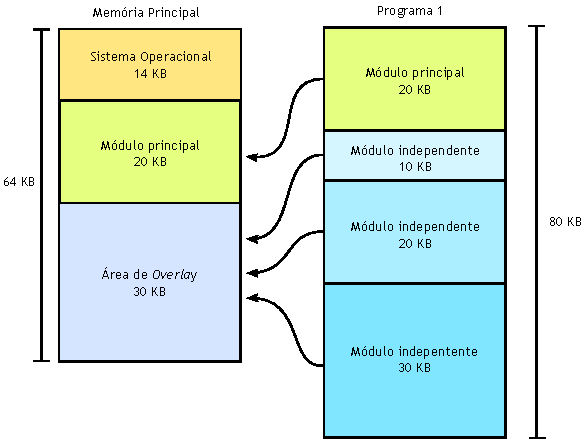
\includegraphics[scale=1]{img/overlay.pdf}
  \caption{Estado da memória principal \label{OverlayPDF}}
\end{figure}

